\begin{landscape}
\chapter{Листинги}
\section{Конфигурационный файл параметров сети Modbus}\label{app:sec:modbus_tag}
    \lstinputlisting[
        language=MyXML,
        caption=Конфигурационный файл для описания множества контроллируемых параетров по промышленному протоколу Modbus
            из раздела \ref{sec:modbus_tag}. Файл разметки приведен в листинге \ref{lst:modbus_tags_example_configs},
        label=lst:modbus_tags_example]
            {Dissertation/listings/xml/modbus_tags_example.xml}
\end{landscape}

\section{Конфигурация сценария}\label{app:sec:modbus_scenario_example_diagram}
\lstinputlisting[
    language=MyXML,
    caption=Конфигурационный файл примера сценария развития событий (см. рисунок \ref{fig:modbus_scenario_example_diagram}),
    label=lst:modbus_scenario_example_diagram]
        {Dissertation/listings/xml/modbus_tags_example_scenario.xml}

\begin{landscape}
\section{XML схемы}\label{app:sec:xsd}
    \lstinputlisting[
        language=MyXML,
        caption=\todo{modbus scheme},
        label=lst:modbus_tags_example_configs]
            {Dissertation/listings/xsd/modbus_tags_configs.xsd}
    
    \lstinputlisting[
        language=MyXML,
        caption=\todo{modbus scenario scheme},
        label=lst:modbus_tags_scenario_configs]
            {Dissertation/listings/xsd/modbus_tags_scenario_configs.xsd}        
\end{landscape}

\begin{landscape}
    \section{Онтология модели АНПА}\label{app:sec:anpa_owl}
    \lstinputlisting[
        language=MyXML,
        caption=Описание онтологии на языке \todo{\texttt{OWL|RDF}},
        label=lst:model_anpa_owl]
            {Dissertation/listings/owl/anpa.owl}
\end{landscape}


\chapter{Свидетельство о государственной регистрации программы для ЭВМ}\label{app:sec:registration}
\begin{center}
    \begin{figure}[hb]
        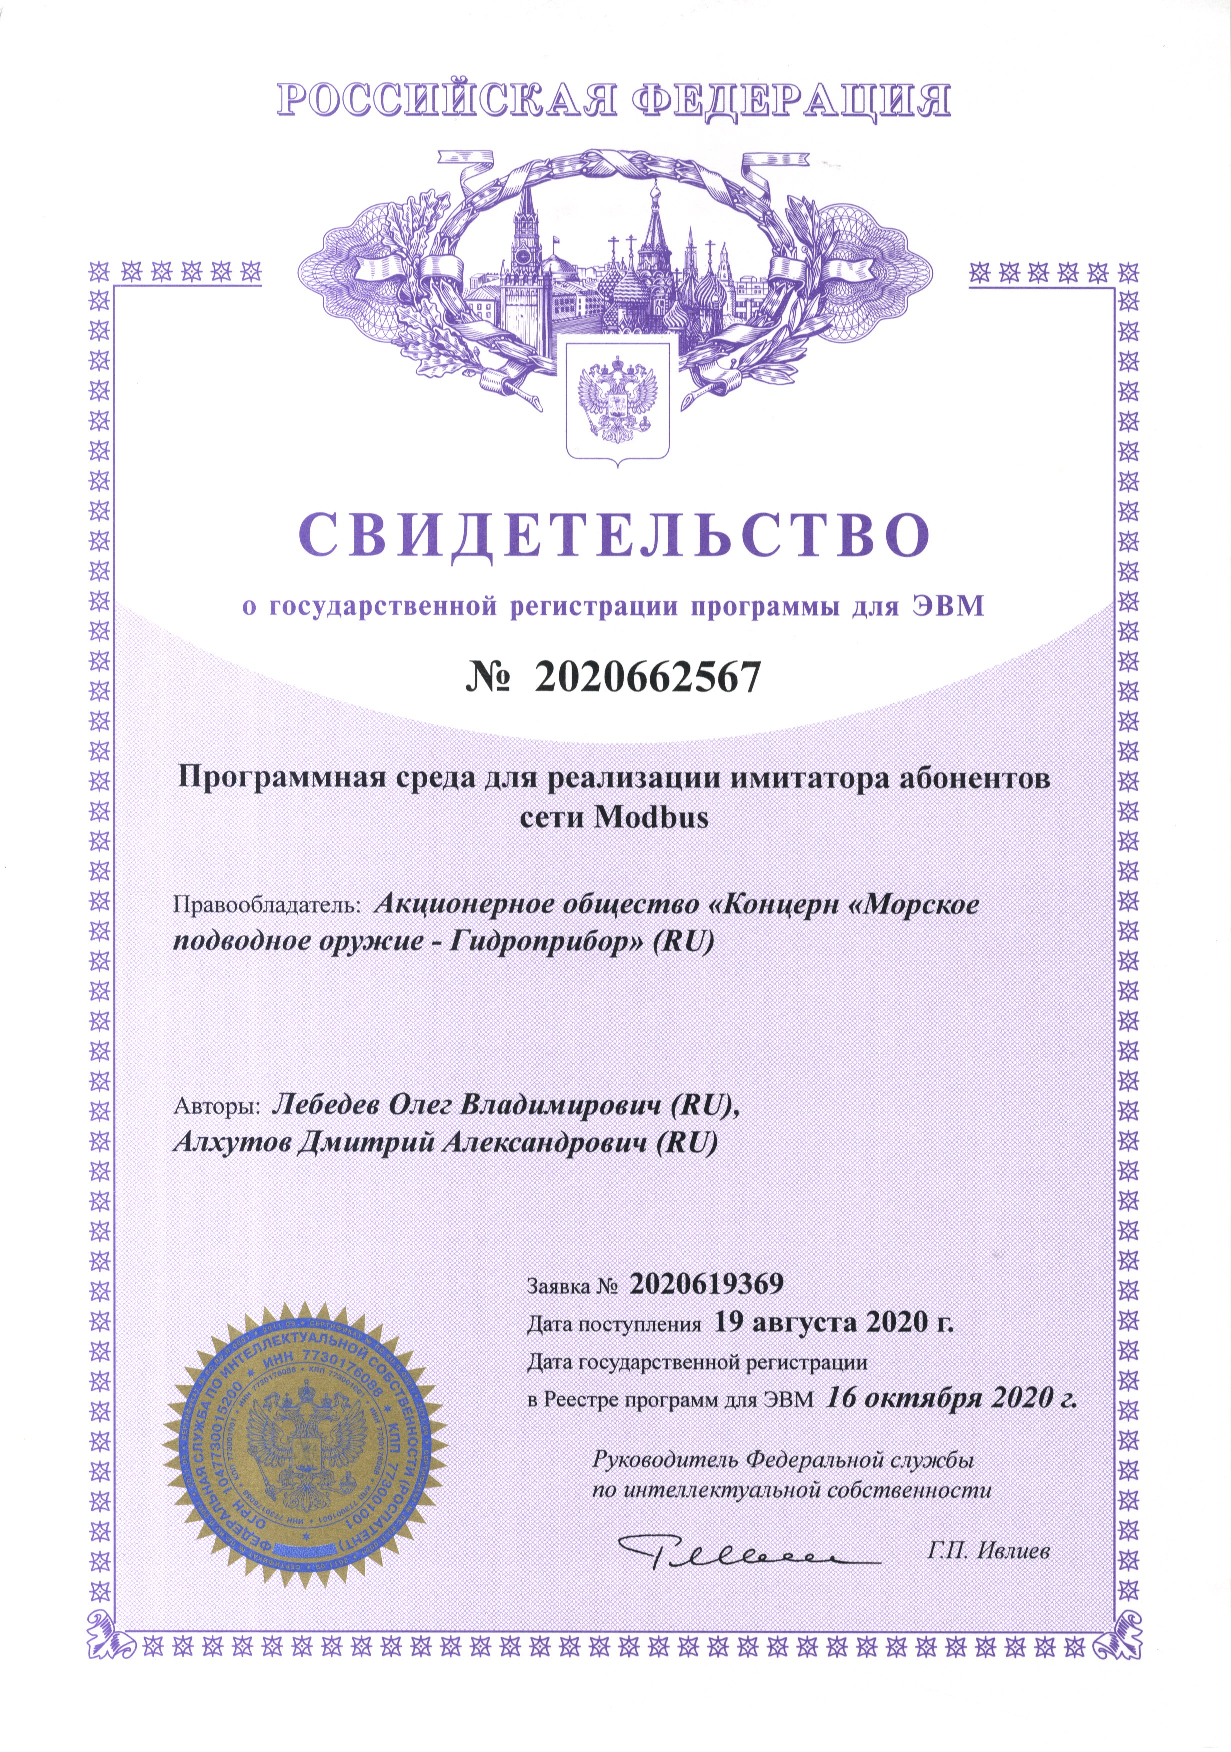
\includegraphics[height=.7\textheight, keepaspectratio]{registration.pdf}
        \caption[Свидетельство о государственной регистрации]
            {Свидетельство о государственной регистрации программы для ЭВМ}\label{app:fig:registration}
    \end{figure}
\end{center}



\chapter{Акт о внедрении}\label{app:sec:implementation}
\begin{center}
    \begin{figure}[hb]
        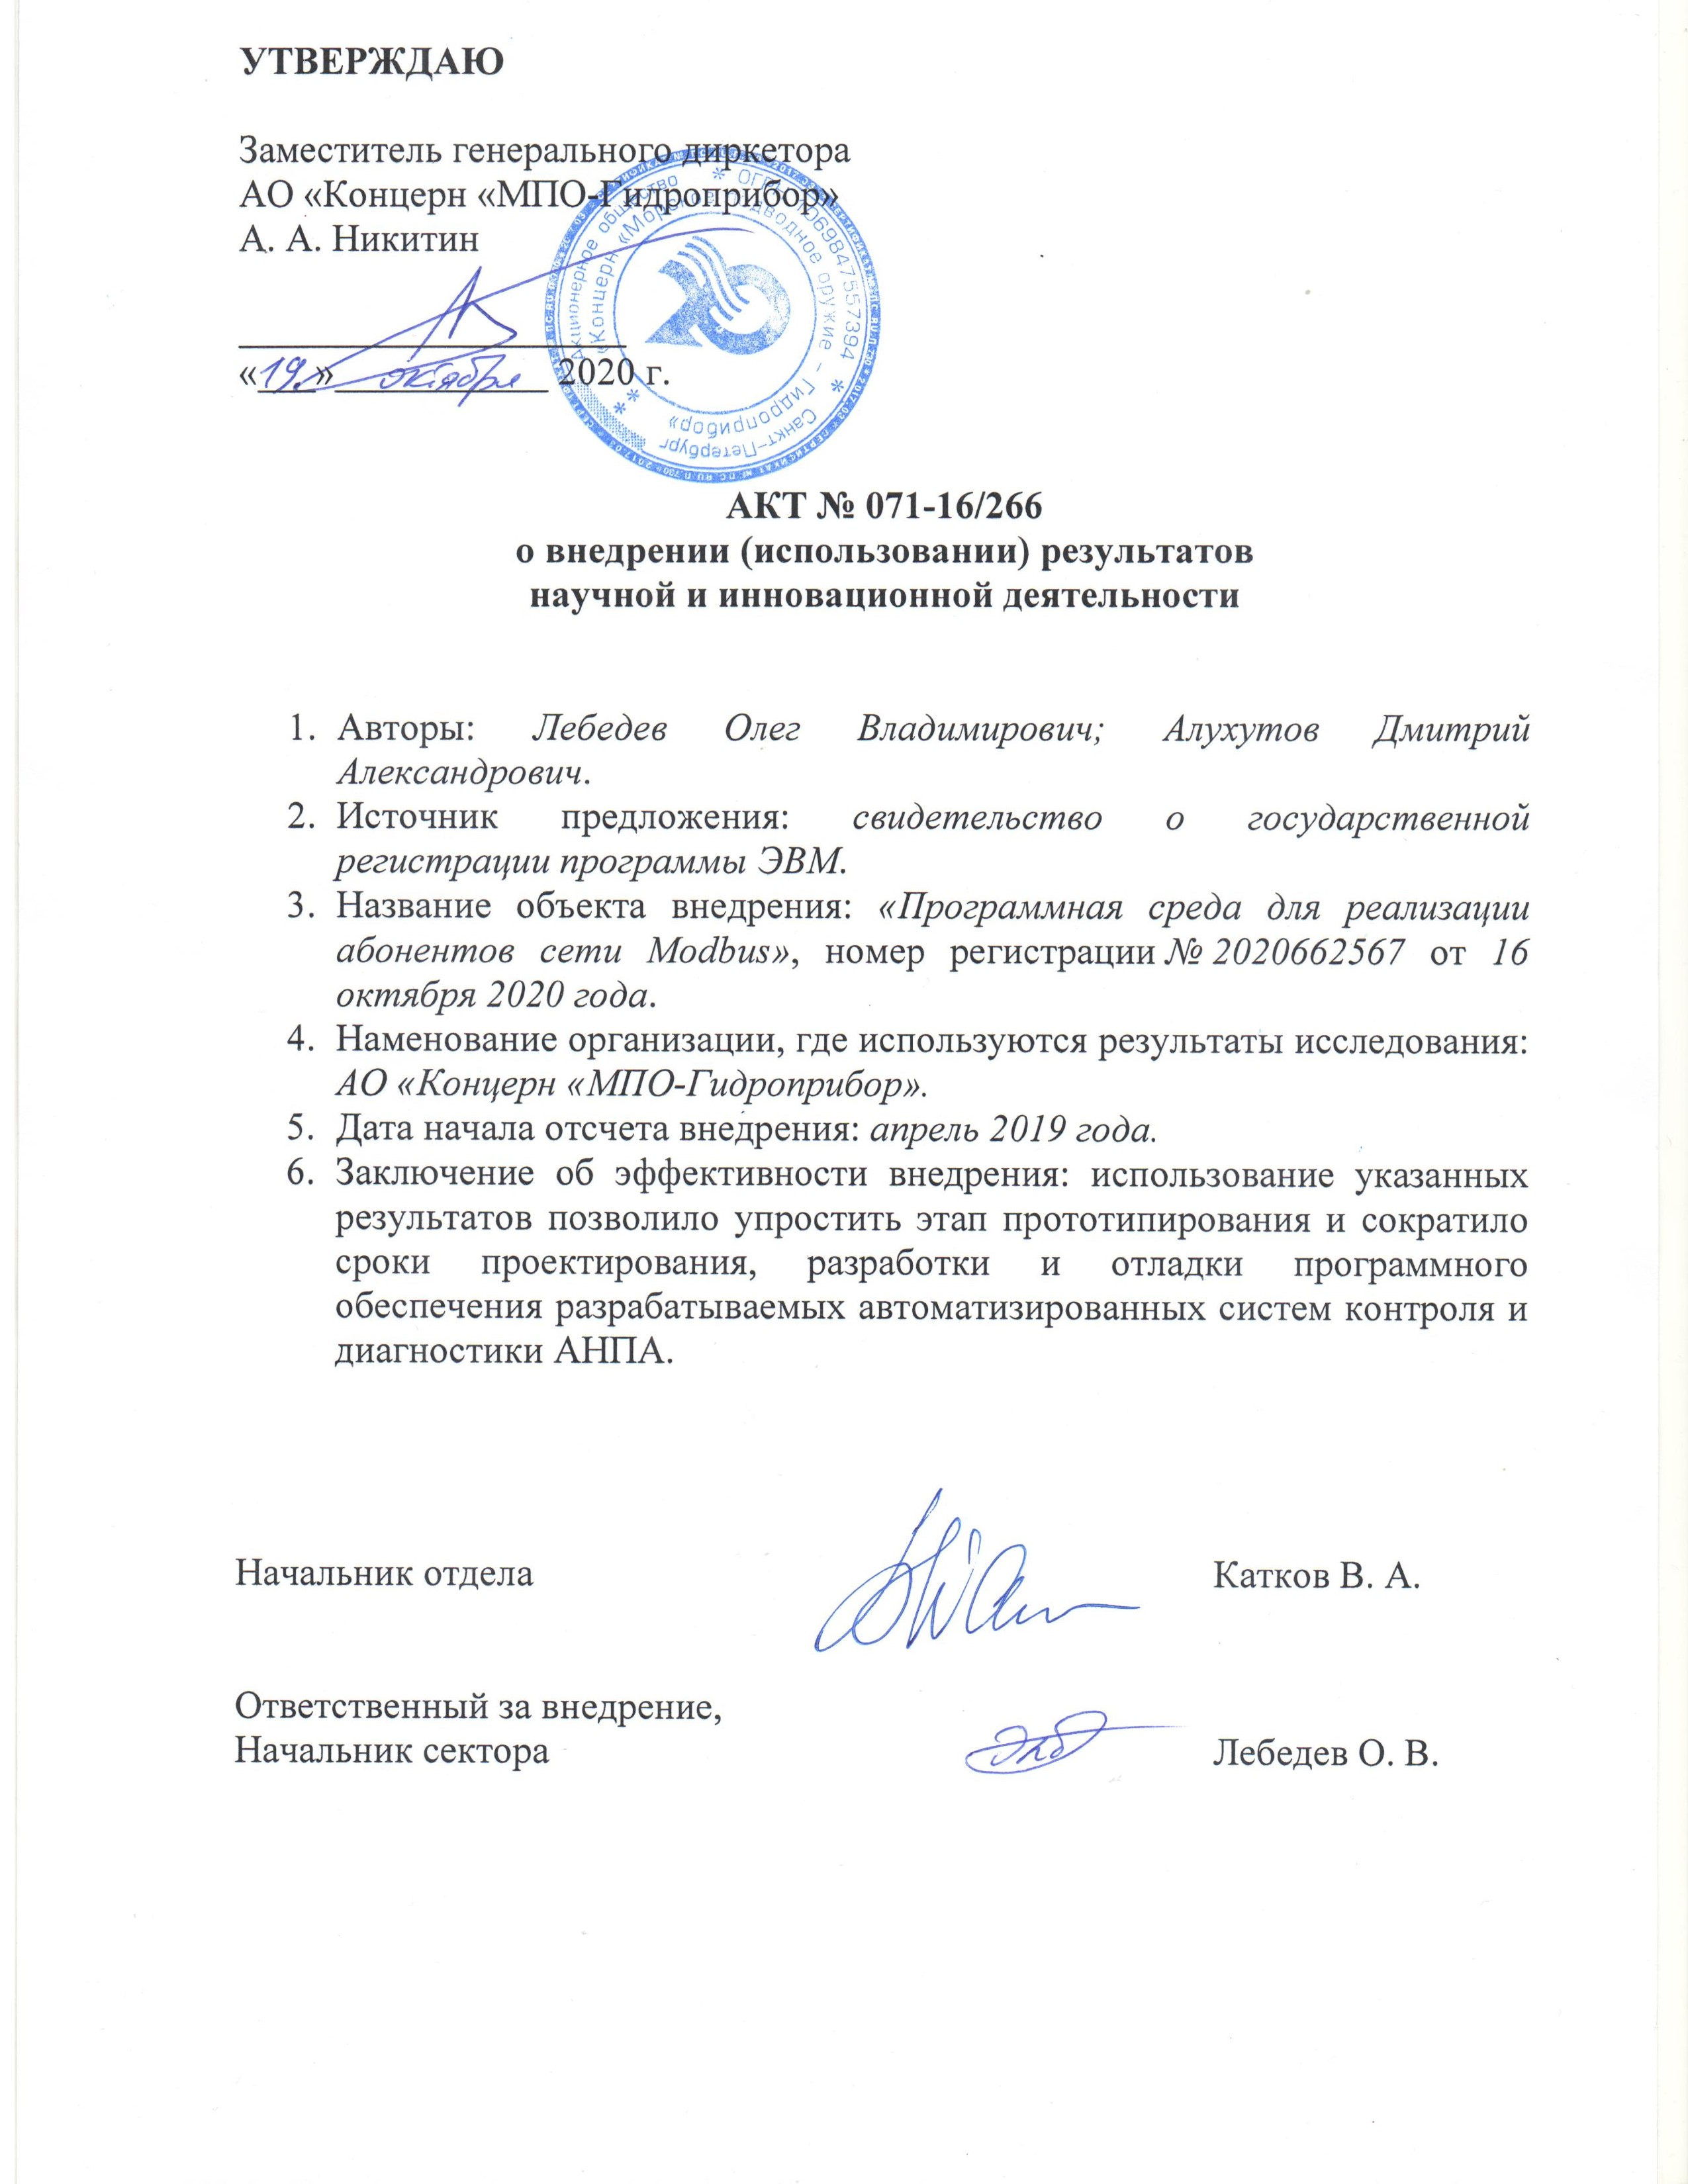
\includegraphics[height=.7\textheight]{implementation}
        \caption[Акт о внедрении]{Акт о внедрении на предприятии \leadingOrganizationTitle}\label{app:fig:implementation}
    \end{figure}
\end{center}

\chapter{Дополнительные рисунки}\label{app:sec:figures}
\begin{center}
    \begin{figure}[hb!]
        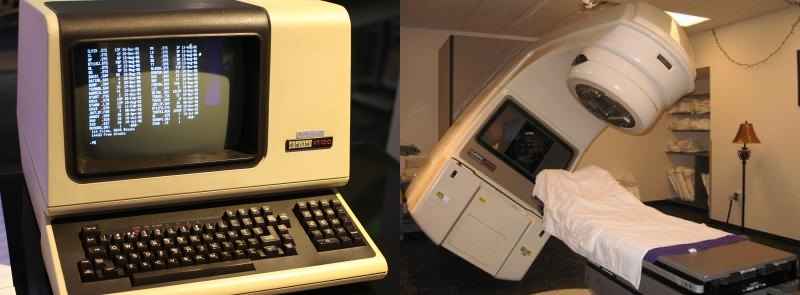
\includegraphics[width=.7\textwidth]{therac25-console}
        \caption[Therac 25]{Therac 25. Консоль оператора показана на рисунке \ref{app:fig:therac25_console}.}\label{app:fig:therac25}
        %
        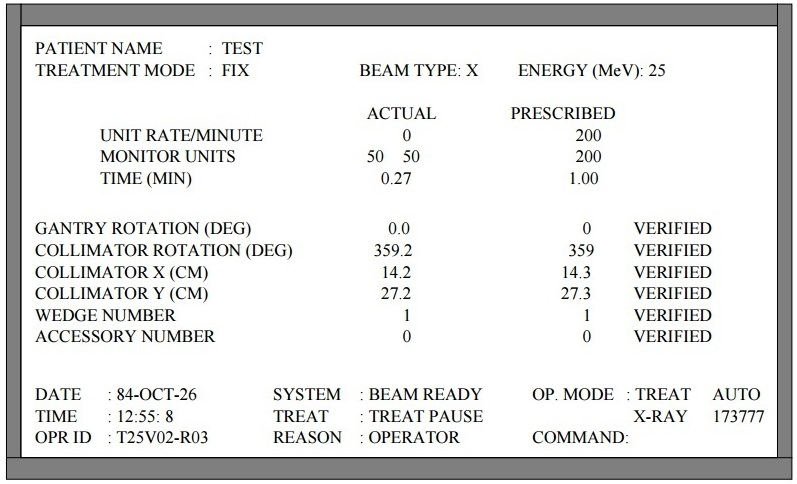
\includegraphics[width=.7\textwidth]{therac25-screenshot}
        \caption[Консоль Therac 25]{Консоль Therac 25.}\label{app:fig:therac25_console}
    \end{figure}
\end{center}
